\vspace{0.5em}
\subsubsection{Frame Aggregator}  
The frame aggregator addresses the inherent sparsity of single radar frames by combining multiple consecutive frames into a denser and more reliable point cloud.  
While aggregation increases both useful information and noise, it ultimately improves object reconstruction, motion estimation, and detection stability.

\paragraph{Single Frame}
Processing a single frame often leads to incomplete or fragmented detections:
\begin{itemize}
    \item Objects may not be fully represented due to the low number of points.
    \item Close objects can merge or be misclassified because of insufficient separation in sparse data.
\end{itemize}

\begin{figure}[!htbp]
    \centering
    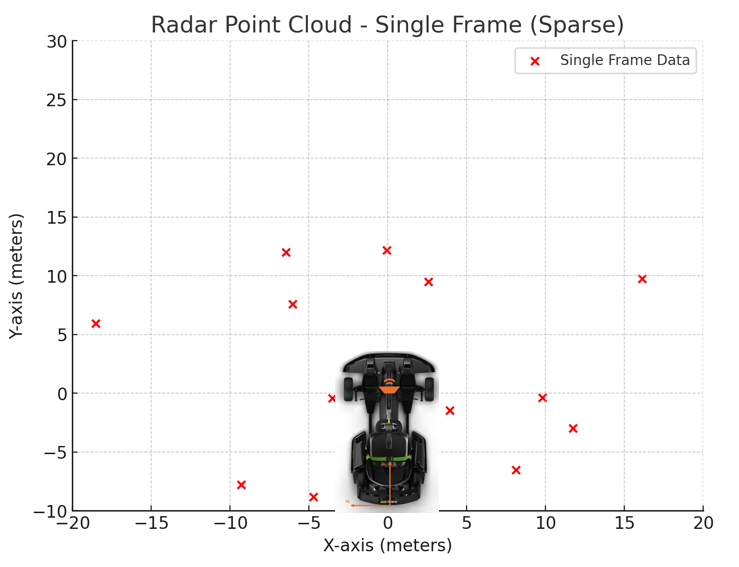
\includegraphics[width=0.5\linewidth]{images/singleframe.png}
    \caption{Single-frame visualization.}
    \label{fig:single_frame}
\end{figure}

This sparsity-induced ambiguity is not a limitation of the clustering algorithms themselves, but a direct consequence of limited raw data.

\paragraph{Multiple Frames}
To mitigate these issues, multiple frames are aggregated in a fixed-size buffer, where older frames are removed as new ones arrive.  
This method increases point cloud density, reduces variance as per the Law of Large Numbers, and stabilizes detections:
\begin{equation}
    \frac{\sigma^2}{N}
    \label{eq:variance_per_sample_size}
\end{equation}

\begin{figure}[!htbp]
    \centering
    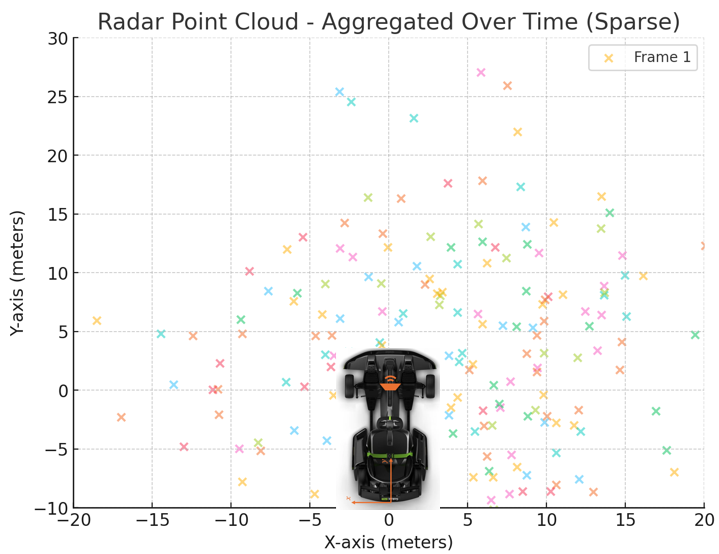
\includegraphics[width=0.5\linewidth]{images/multiframe.png}
    \caption{Multi-frame aggregation visualization.}
    \label{fig:multiframe}
\end{figure}

During experimentation, the number of aggregated frames was varied between 7 and 15.  
A value of 10 frames provided the best balance: enough temporal density to reduce noise and reveal stable structures, while minimizing the persistence of outdated points.  
This configuration was therefore adopted for all subsequent pipeline stages.
